\section{Fundamentação Teórica}

\begin{frame}{Fundamentação Teórica}
    \begin{itemize}
        \item \textbf{Grafos planares} são grafos que podem ser desenhados no plano de forma que suas arestas não se cruzem, exceto nos vértices em que se encontram.
        
        \item \textbf{Coloração de grafos} é um processo de atribuição de cores aos vértices de um grafo de forma que dois vértices adjacentes (conectados por uma aresta) nunca recebam a mesma cor. O objetivo é minimizar o número total de cores utilizadas.
    \end{itemize}
\end{frame}

\begin{frame}{Por que Grafos Planares?}
    \begin{itemize}
        \item Possuem propriedades teóricas bem definidas, como o Teorema das Quatro Cores, o que fornece um limite superior teórico.
        
        \item São estruturas \textit{esparsas}, o que os torna ideais para testar a eficiência dos algoritmos em contextos práticos.
    \end{itemize}
\end{frame}

\begin{frame}{Como os Grafos Planares foram gerados?}
\begin{itemize}
    \item \textbf{Construção Inicial}
    \begin{itemize}
        \item Define-se \( k = \lfloor \sqrt{n} \rfloor \)
        \item Cria-se uma malha retangular com \( k \times k \) vértices
        \item Resultado: grafo \textbf{planar}, com até \( k^2 \) vértices
    \end{itemize}

    \item \textbf{Quando Remove Vértices} \hfill (se \( k^2 > n \))
    \begin{itemize}
        \item Remove-se os \( k^2 - n \) vértices excedentes
        \item Também são removidas as arestas incidentes a eles
        \item A planaridade é preservada, pois não há cruzamento novo
    \end{itemize}

    \item \textbf{Quando Adiciona Vértices} \hfill (se \( k^2 < n \))
    \begin{itemize}
        \item Adiciona-se \( n - k^2 \) novos vértices ao grafo
        \item Cada novo vértice é conectado a um vértice existente com grau \( < 4 \)
        \item Esse limite evita aglomeração e mantém a planaridade
    \end{itemize}
\end{itemize}
\end{frame}

\begin{frame}{Importância da geração sintética}
    \begin{itemize}
        \item Permite o controle do número de vértices e reprodutibilidade dos testes.
        
        \item Garante que o grafo está de acordo com os \textit{limites teóricos esperados}, como não ultrapassar o grau 4 para manter a planaridade.
        
        \item Evita depender de grafos reais com ruído ou propriedades indesejadas.
    \end{itemize}
\end{frame}

\begin{frame}{Cenário real: Alocação de frequências em torres de celular}
    \begin{columns}[T] % O [T] alinha as colunas pelo topo
        
        % Coluna da Esquerda (Texto)
        \begin{column}{0.6\textwidth}
            Imagine uma cidade com várias torres de celular instaladas em diferentes bairros. 
            Cada torre transmite sinal em uma certa frequência. 
            Se duas torres \textbf{próximas} usarem a mesma frequência, os sinais podem \textbf{interferir} entre si, prejudicando a conexão.
        \end{column}
        
        % Coluna da Direita (Imagem)
        \begin{column}{0.4\textwidth}
            % Certifique-se de que o caminho para a imagem está correto
            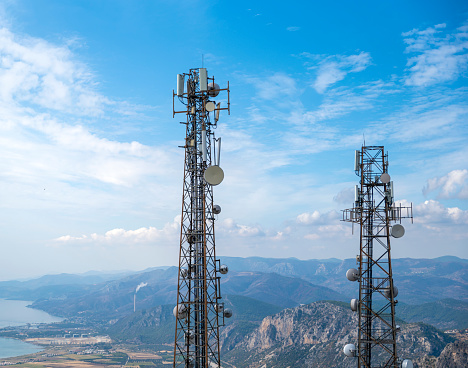
\includegraphics[width=\textwidth]{figures/power_lines.jpg}
        \end{column}
        
    \end{columns}
\end{frame}

\begin{frame}{Como modelar isso com grafos?}
    \begin{itemize}
        \item Cada torre de celular é representada por um \textbf{vértice}.
        
        \item Se duas torres estão próximas (na mesma região de cobertura), conectamos os vértices com uma \textbf{aresta}, porque elas \textbf{não podem usar a mesma frequência}.
        
        \item Atribuímos uma \textbf{``cor''} para cada vértice, representando uma \textbf{frequência de transmissão}. O objetivo é \textbf{minimizar} o número de frequências diferentes, mas garantindo que torres próximas \textbf{não tenham a mesma cor}.
    \end{itemize}
\end{frame}